\documentclass{article}
\usepackage{amsmath}
\usepackage{tikz} 
\usepackage[a4paper]{geometry}
\usepackage{hyperref} 
\usepackage{fancyhdr}
\pagestyle{fancy}
\lhead{Abschnittsweise definierte Funktionen}
\rhead{April 2025}
\begin{document}
\section{Abschnittsweise definierte Funktionen} 
Eine Abschnittsweise definierte Funktion ist eine Funktion, welche an unterschiedlichen Positionen aus verschiedenen Gleichungen zusammengesetzt ist. In einer geschweiften Klammer werden untereinander die Formeln der jeweiligen Abschnitte, gefolgt von einem Komma und dem Definitionsbereich des Abschnitts aufgeschrieben. Dies sieht beispielshaft so aus.
\[
f(x) =
\begin{cases} 
 -x, & \text{für } x < 0 \\ 
 x, & \text{für } x \ge 0
\end{cases}
\] 
Die Stellen, an welchen die Funktion von der einen zu anderen Gleichung übergeht, in die Fall bei $x=0$, ist die Nahtstelle. 
 
\subsection{Stetigkeit}
Eine Funktion ist stetig, wenn der Funktionsgraph eine durchgängige Linie, ohne einem Sprung, ist. Dies kann entweder visuell am Graphen oder mathematisch festgestellt werden. \newline
Somit ist eine Funktion f an der Nahtstelle $x_0$ stetig, wenn der Funktionswert an der Nahtstelle dem Limit an der Nahtstelle gleich ist, in allen Fällen wenn
\[
 \lim_{x \to x_0^-} f(x) = f(x_0) = \lim_{x \to x_0^+} f(x)
\]
An einem Beispiel einer stetigen und einer nicht stetigen Funktion
\begin{center} 
 \setlength{\tabcolsep}{1cm} 
 \begin{tabular}{c c}
  stetig
  &
  nicht stetig 
  \vspace{0.5cm}  
  \\ 
  \begin{tikzpicture}
    \draw[blue, thick, domain=-2^0.5:0, samples=100] 
            plot (\x, {\x*\x});
    \draw[blue, thick, domain=0:2, samples=100] 
            plot (\x, 0.5*\x);  
  
    \draw[->] (-2, 0) -- (2, 0) node [above left] {$x$}; 
    \draw[->] (0, -1) -- (0, 2) node [below right] {$y$};
  \end{tikzpicture}  
  &
  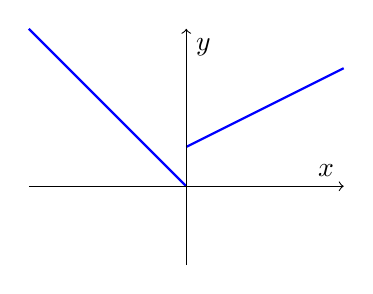
\begin{tikzpicture}
    \draw[blue, thick, domain=-2:0, samples=100] 
            plot (\x, {-\x});
    \draw[blue, thick, domain=0:2, samples=100] 
            plot (\x, 0.5+0.5*\x);  
  
    \draw[->] (-2, 0) -- (2, 0) node [above left] {$x$}; 
    \draw[->] (0, -1) -- (0, 2) node [below right] {$y$};
  \end{tikzpicture} 
  \vspace{0.5cm} 
  \\ 
  $\lim\limits_{x \to x_0^-} f(x) = 0 = 0 = \lim\limits_{x \to x_0^+} f(x)$
  &
  $\lim\limits_{x \to x_0^-} f(x) = 0 \neq 1 = \lim\limits_{x \to x_0^+} f(x)$ 
 \end{tabular}
\end{center} 
 
\subsection{Differenzierbarkeit} 
Eine Funktion ist differenzierbar, wenn der Funktionsgraph eine glatte Linie ohne Knick darstellt und stetig ist. Auch dies kann entweder visuell am Graphen oder mathematisch festgestellt werden. \newline
Somit ist eine Funktion f an der Nahtstelle $x_0$ differenzierbar, wenn es genau eine definierte Steigung hat, also
\[
 \lim_{x \to x_0} \frac{f(x)-f(x_0)}{x - x_0}
\]
existiert, das heißt der limes von beiden Seiten aus den gleichen Wert hat.
An einem Beispiel einer stetigen und einer nicht stetigen Funktion
\begin{center} 
 \setlength{\tabcolsep}{0.8cm} 
 \begin{tabular}{ccc}
  differenzierbar 
  & 
  nicht differenzierbar
  &
  nicht differenzierbar
  \vspace{0.5cm}  
  \\ 
  \begin{tikzpicture}
    \draw[blue, thick, domain=-1^0.5:0, samples=100] 
            plot (\x, {0.5+(\x)^2});
    \draw[blue, thick, domain=0:1.5, samples=100] 
            plot (\x, 0.5);  
  
    \draw[->] (-1.5, 0) -- (1.5, 0) node [above left] {$x$}; 
    \draw[->] (0, -1) -- (0, 1.5) node [below right] {$y$};
  \end{tikzpicture} 
  &
  \begin{tikzpicture}
    \draw[blue, thick, domain=-1:0, samples=100] 
            plot (\x, {-\x+0.5});
    \draw[blue, thick, domain=0:1.5, samples=100] 
            plot (\x, 0.5);  
  
    \draw[->] (-1.5, 0) -- (1.5, 0) node [above left] {$x$}; 
    \draw[->] (0, -1) -- (0, 1.5) node [below right] {$y$};
  \end{tikzpicture} 
  &
  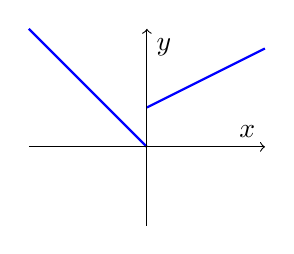
\begin{tikzpicture}
    \draw[blue, thick, domain=-1.5:0, samples=100] 
            plot (\x, {-\x});
    \draw[blue, thick, domain=0:1.5, samples=100] 
            plot (\x, 0.5+0.5*\x);  
  
    \draw[->] (-1.5, 0) -- (1.5, 0) node [above left] {$x$}; 
    \draw[->] (0, -1) -- (0, 1.5) node [below right] {$y$};
  \end{tikzpicture} 
  \vspace{0.5cm} 
  \\
  stetig, Wert für
  & 
  kein Wert für
  &
  nicht stetig, deshalb
  \vspace{0.2cm} 
  \\
  $\lim\limits_{x \to x_0} \dfrac{f(x)-f(x_0)}{x - x_0} = 0$
  &
  $\lim\limits_{x \to x_0} \dfrac{f(x)-f(x_0)}{x - x_0}$
  &
  nicht differenzierbar 
 \end{tabular} 
\end{center}
 
\subsection{Funktionen Verbinden}
\begin{minipage}{\dimexpr\linewidth-4cm}
 Soll eine Funktion $f$ aufgestellt werden, welche zwei andere gegebene Funktionen $t_1$ und $t_2$ verbindet, gegebenenfalls ohne einem Knick, muss diese Funktion unbedingt an den Nahtpunkten stetig und eventuell differenzierbar sein.
 
 Um dies zu erfüllen muss die neue Funktion $t$ an den Nahtpunkten einen Punkt mit den jeweiligen anderen Funktionen teilen. 
\end{minipage}
\hfill
\begin{minipage}{4cm}
 \center
 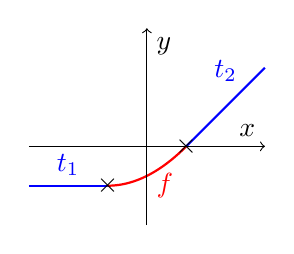
\begin{tikzpicture}
 \draw[blue, thick, domain=-1.5:-0.5, samples=100] plot (\x, -0.5);
 \draw (-1, -0.5) node [blue, above] {$t_1$};
 \draw[blue, thick, domain=0.5:1.5, samples=100] plot (\x, {\x-0.5});
 \draw (1, 0.7) node [blue, above] {$t_2$};
 
 \draw[red, thick, domain=-0.5:0.5, samples=100] plot (\x, {(\x+0.5)^2/2-0.5});
 \draw (0, -0.5) node [red, right] {$f$};
  
 \draw (-0.5, -0.5) node [] {$\times$};
 \draw (0.5, 0) node [] {$\times$}; 
 \draw[->] (-1.5, 0) -- (1.5, 0) node [above left] {$x$}; 
 \draw[->] (0, -1) -- (0, 1.5) node [below right] {$y$};
 \end{tikzpicture}  
\end{minipage} 
Liegt beispielsweise $t_1$ bei der Nahtstelle $x_1$ so muss auch $f(x_1)=t_1(x_1)$ gelten. 
Um differezierbar zu sein müssen die Funktionen an der gleichen Stelle auch die Gleiche Steigung haben, sodass $f'(x_1)=t_1'(x_1)$. Gleiches gilt jeweils auch für die andere Nahtstelle.
Wie eine Funktion mit diesen Bedingungen aufgestellt wird ist im Kapital \hyperref[Steckbriefaufgaben]{Steckbriefaufgaben} beschrieben.
\end{document}  
 
